\documentclass[a4paper]{article}
\usepackage{graphicx} \usepackage{caption} \usepackage{pdfpages} \usepackage{pdflscape} \usepackage[margin=0.8in]{geometry} \usepackage{fancyhdr} \usepackage{pdfpages} \usepackage{lastpage}
\begin{document}
\pagestyle{fancy}
\fancyhead[LO,LE]{Project Plan, v1.3, Release}
\fancyfoot[C]{Aberystwyth University / Computer Science}
\fancyfoot[RO, LE] {\thepage\ of \pageref{LastPage}}
\begin{center}
\textsc{\LARGE The Software Development Life Cycle}\\[1.5cm]

\includegraphics[width=0.15\textwidth]{img/monster.png}\\[1.5cm]    
\textsc{\Large Monster Mash - Project Plan}\\[0.5cm]

\begin{minipage}{0.8\textwidth}
\begin{flushleft} \large
\emph{Authors:}\\
James \textsc{Bowcott}\\
Simon \textsc{Evans}\\
Craig \textsc{Heptinstall}\\
Aled \textsc{Morgan}\\
Scott \textsc{Roe}\\
Kami \textsc{Tacickaja}\\
\end{flushleft}
\end{minipage}
\vspace{8 mm}

\begin{minipage}{0.8\textwidth}
\begin{flushleft} \large
\emph{Task ID:}
SE\_03\_OVERVIEW\\
\end{flushleft}
\end{minipage}
\vspace{8 mm}

\begin{minipage}{0.8\textwidth}
\begin{flushleft} \large
\emph{Version:}
1.3\\
\end{flushleft}
\end{minipage}
\vspace{8 mm}

\begin{minipage}{0.8\textwidth}
\begin{flushleft} \large
\emph{Status:}
Release\\
\end{flushleft}
\end{minipage}
\vspace{8 mm}

\begin{minipage}{0.8\textwidth}
\begin{flushleft} \large
Department of Computer Science\\
Aberystwyth University\\
Aberystwyth\\
Ceredigion\\
SY23 3DB\\
\end{flushleft}
\end{minipage}
\vfill
{\large \today}
\end{center}
\clearpage
\setlength\parindent{0pt}

%TOC

\tableofcontents
\clearpage

%Aled - Intro

\section{Introduction}

\subsection{Purpose of this Document}

This document describes the design specification for the Software Engineering Group Project 2012-2013. It should be read in the context of the Group Project, taking into account the details of the group project assignment and the group project Quality Assurance (QA) Plan. [1]

\subsection{Scope}

The document should provide a design for the implementation in relation to the Requirements Specification. All members of the project should read this document.

\subsection{Objectives}

The objectives are this document are:

\begin{itemize}
\item To depict the function of the Monster Mash project with use of Use Case diagrams.
\item To provide User Interface details.
\item To provide an implementation of the project schedule.
\item To collate a suitable risk analysis and describe procedures to follow if any such risks occur.
\end{itemize}
\clearpage

%James - overview

\section{Overview of proposed system}
The project requirements specification outlines that the Monster Mash game should be implemented in a server-client architecture over the World Wide Web, where the application resides and runs on a web application server, with which the user (client) interacts using a standard web browser.\\

The software stack chosen for this project consists of the following:
\begin{itemize}
\item \textbf{Java EE}
\item \textbf{GlassFish} Java EE web application server
\item \textbf{PostgreSQL} SQL RDBMS server
\item \textbf{SVN} software versioning and revision control system
\end{itemize}

These software solutions are both open-source, and so are free to use, and are already provided by the university's servers.\\

An important condition in the design of the system is that it should be able to be deployed to, run and maintained on servers provided by the university. The system should not have to rely on services provided by a third-party to be in service. Firstly, because there can not be any costs in the system's operation, but even free services, such as Google's App Engine, may force development against proprietary API's, forcing vendor lock in, and introduce risks of downtime which would be outside of our control.

\subsection{Java EE}

The game logic and its presentation will be developed in Java EE Servlets. The specification requires that the application be written using Java. Java Enterprise Edition is the standard API for delivering dynamic web applications written in Java. A Java EE application, or Servlet, is run on the server, rather than the user's machine.\\

It works a lot like a standard HTTP web service. A user requests a page, the server responds to that request and a page is generated and sent to the client, which is displayed in the users web browser. This is better than an applet, which is basically a Swing application running inside the browser, as it does not require Java to be installed on the client's machine. All they need is a standard web browser.

\subsection{GlassFish}

Java EE applications are run in a web application server, which works like a standard HTTP web server, handling HTTP requests, but refers those requests to a Servlet, which it runs and handles various users sessions to.\\

There are several Java EE servers available. GlassFish was chosen not just because it is already set up on university servers, but because it provides a lot of features such as RDBMS connection management, and support for numerous API's which aid in the development, deployment and integration of Java Servlets.

\subsection{PostgreSQL}

The application will need to store user data, such as user details, monsters, friends etc.
A relational database is best suited for this as it extends the Object-Oriented approach of a Java application model.
Java EE has a strong API for persisting data to SQL, so this was chosen over other methods of data persistence.
The Java Servlet interfaces with the server through a standard socket connection, and acts as a controller between state in the application and data persistence in the database.

\subsection{SVN}

The code base for the project needs to be managed in a version control system. Using version control provides not only a centralised store for source code, but also allows easier collaboration, aids in keeping track of changes and versions, and provides rollback functionality.\\

There are a number of version control systems available for use. We have decided to use Apache Subversion, a.k.a. SVN. SVN is widely supported by Integrated Development Environments, and applications which integrate SVN into the operating system. It provides all of the functionality mentioned earlier, and is available pre-setup on university servers, so hosting is not an issue.\\

The advantages that version control brings to code will also be applied to documentation, as this is an ideal solution for collaboration, versioning and storage of documentation.

\subsection{Server-Server Communication}

Another requirement is that the application should be able to communicate with other group's implementations of the game. For this, our server needs to be able to communicate with other servers using some defined server-server communication standard. This standard should require that each group's server should implement a common interface, allowing servers to share information such as friend requests, fight requests etc.\\

Defining a standard should allow each group to make their own implementation of that standard, instead of having one group complete an implementation and then force others to use that implementation. The standard has yet to be defined, but a task force group has been set up to open discussions on a standard.
\clearpage

%Craig - UML

\section{UML}
\subsection{UML Diagrams}
In this section of the document, we will now display a set of use cases
designed for the programs aimed user interaction possibilities. We will
split up these different possible functionalities into a set of diagrams
which break down activities such as registering and logging into the
program, along with having battles/ trades/ breeds with other users on the
same or other servers. This section of the document follows the guidelines
and instructions laid out in the project plan specification standards
document [2] defining the provision of use
case diagrams.

\begin{center}
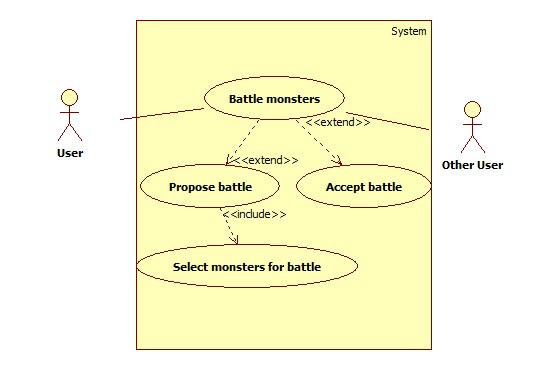
\includegraphics[width=\textwidth]{img/UseCaseBattle.jpg}
\captionof{figure}{UML for Battle class}
The breed monsters diagram displayed above shows similar layout to the previous diagram, but has more detail when it comes to battling monsters. But similar to the adding of friends use case, this one shows that users should be able to propose and accept battles within the battling of monsters command. The difference in this diagram is that users also have another broken down use case of selecting the monsters, where they will choose what monster they want to use within a battle. Breaking this diagram into more detail such as this one, will provide us with a better idea of what classes\ methods will need to be implemented.

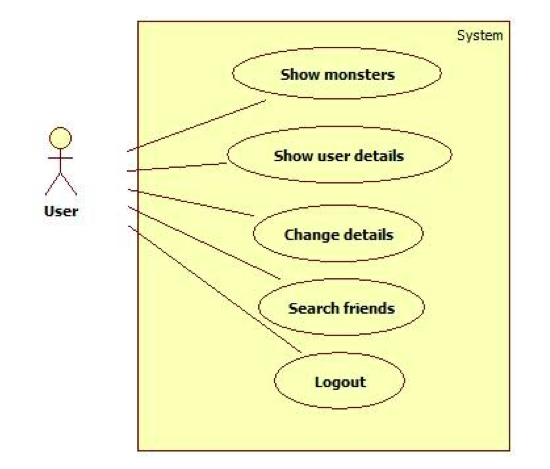
\includegraphics[width=\textwidth]{img/UseCaseLScreen.jpg}
\captionof{figure}{UML for Login Screen}
In the second figure displayed, this represents the users’ first options after logging into the system. The general idea of this diagram shows that users should be able to bring up a list of their own monsters, display their data, and allow the option to change details, search friends and logout. Having a good number of options available to the user at this stage will mean easier accessibility around the system whilst attempting to not being too clustered by offering too options giving a messy feel. On top of these possible uses on the homepage of the site, we could also provide some basic statistics or information on recent battles/ trades etc. for the user.

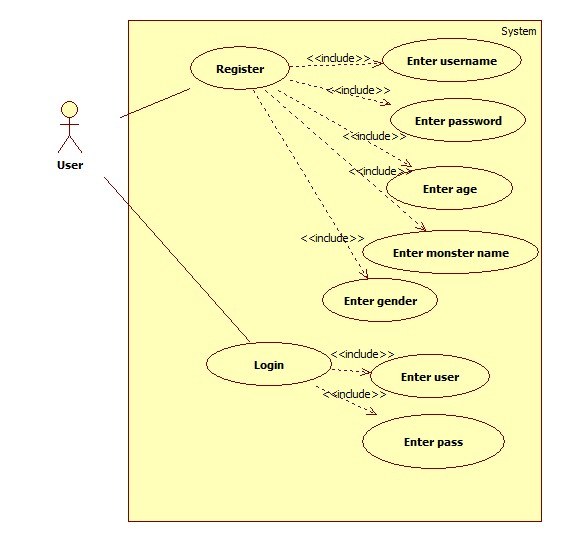
\includegraphics[width=\textwidth]{img/UseCaseHome.jpg}
\captionof{figure}{UML for Home class}
Figure 3 illustrates the first of our use case diagrams for the proposed system, and in this detailed example, shows the use of the login page when users first navigate to our web application. As you can see, they should be presented with two options, one to login if they are a previous user, and one option allowing them to register as a new user. In this diagram we have broken down and chosen to show the options within each of these, for example in the login section, the user should be able to simply enter their username and password in order to login. We have shown this with an ‘include’ link to each of these options. As for the registration break down within this diagram, you can see the use case has multiple options the user can perform from creating a username, password and monster name, to entering their age/ gender. This diagram is one of the most important of the use cases, as it defines what users information and layout of starting the application will be.

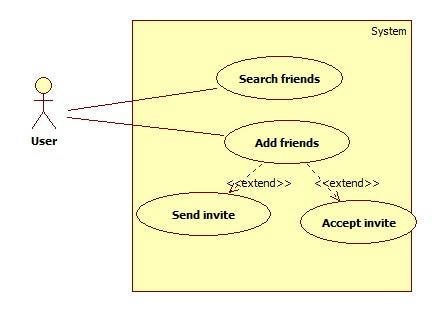
\includegraphics[width=\textwidth]{img/UseCaseFriends.jpg}
\captionof{figure}{UML for Friends class}
This use case gives an idea of how we aim to allow users to add and search friends within the game, broken down again into the sending of an invite and accepting an invite. Using the extend arrows on this diagram displays the multiple uses that adding a friend on the game can involve.

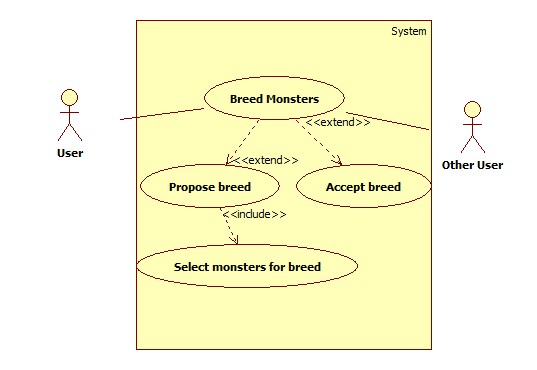
\includegraphics[width=\textwidth]{img/UseCaseBreed.jpg}
\captionof{figure}{UML for Breed class}

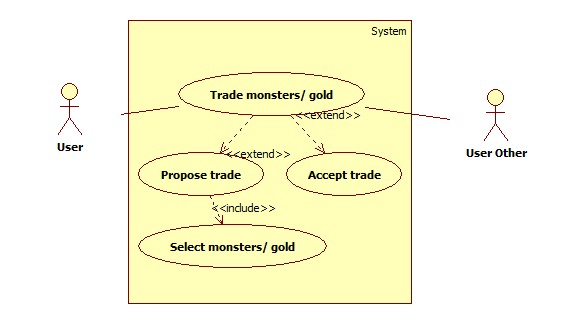
\includegraphics[width=\textwidth]{img/UseCaseTrade.jpg}
\captionof{figure}{UML for Trade class}
In the penultimate use case diagram, and similarly the final diagram, both follow the same layout as the previous, displaying the users’ options of trading/ breeding monsters. And by breaking down the two again to the proposal/ acceptance of decisions of users, it helps us and the client understand what options will be implemented later on in the project. Also similar to the previous diagram, it shows that users should be allowed to choose the monsters for breeding/ trading. This is an obvious use that users should be allowed.
\end{center}
\clearpage

%Kami - UI

\section{User Interface Design}
\subsection{UI Design}

The starting screen must allow the user to either login or register - I thought the best solution would be both options displayed on one screen with both possibilities easily approachable rather than choosing one and being redirected to another screen.\\

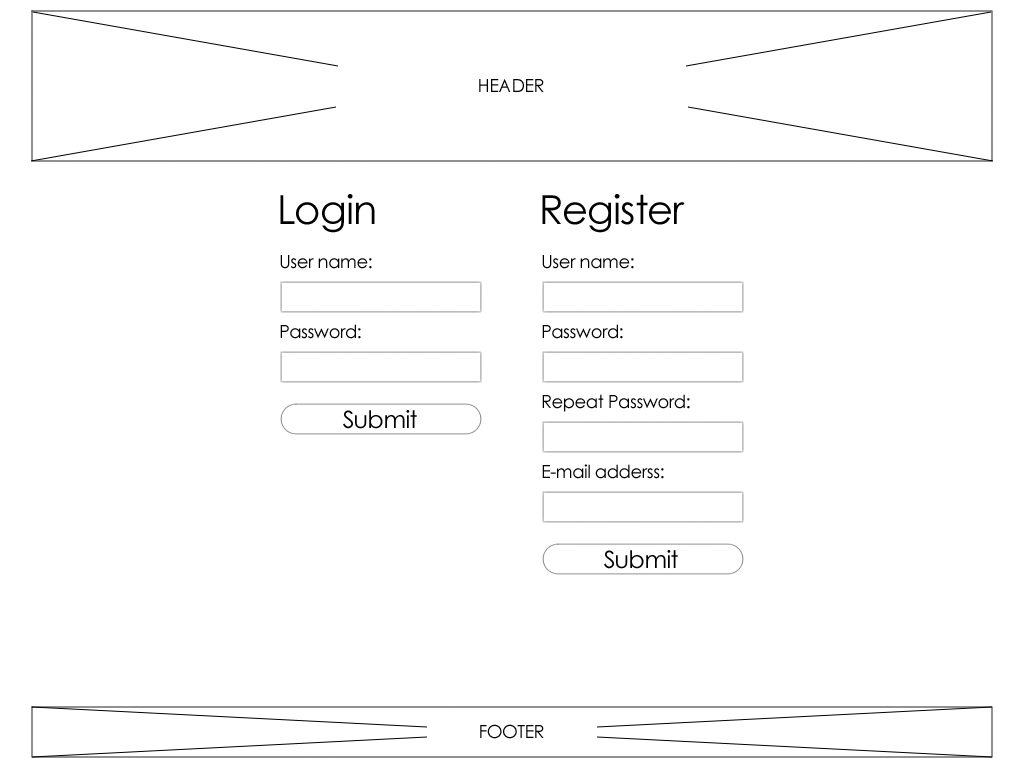
\includegraphics[width=\textwidth]{img/UI17.jpg}
\clearpage

If the user has chosen the register option they will be moved to a redirected screen or a pop-up. Registration fields should be reset as soon as the submit button is activated.\\
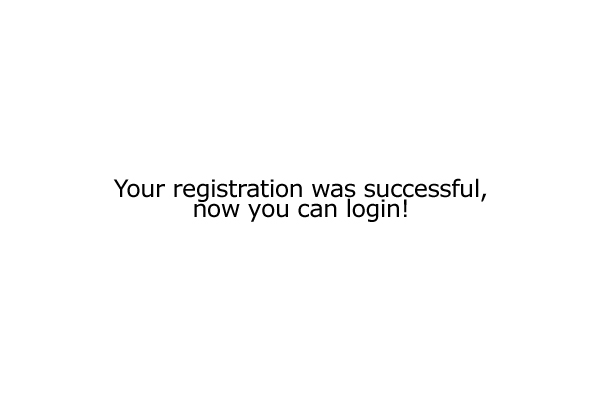
\includegraphics[width=\textwidth]{img/UI18.jpg}
\clearpage

Once the user is registered, he/she can login and the home page will be displayed. Here, the user can see their short profile, all monsters listed underneath, all friends who are currently offering to sell or breed their monsters and all challenge requests received from their friends.\\

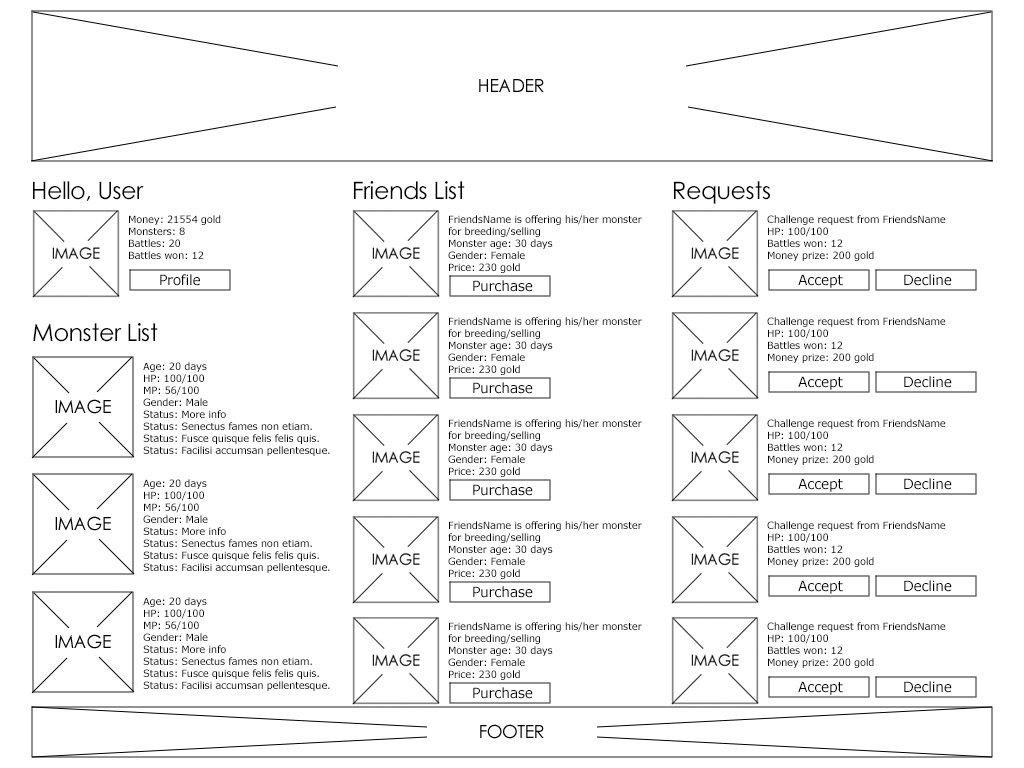
\includegraphics[width=\textwidth]{img/UI3.jpg}

Here the user has a few options. Users can purchase monsters in which case he/she has two possible options. Either the purchase will be successful or the purchase will fail due to lack of money. The user can also accept or decline battle requests - if the user clicks 'Decline', the page will refresh and the battle request will disappear. If the user accepts the request, however, they will be able to choose which monster they want to use in battle. Once the battle is over, the user will get a message to confirm wether or not they have won - in the case of winning, the prize and monster status will be displayed.
\clearpage

The user should also be able to check their profile by clicking the 'Profile' button. By default it will take them to Profile page where the user can see all their monsters listed.\\

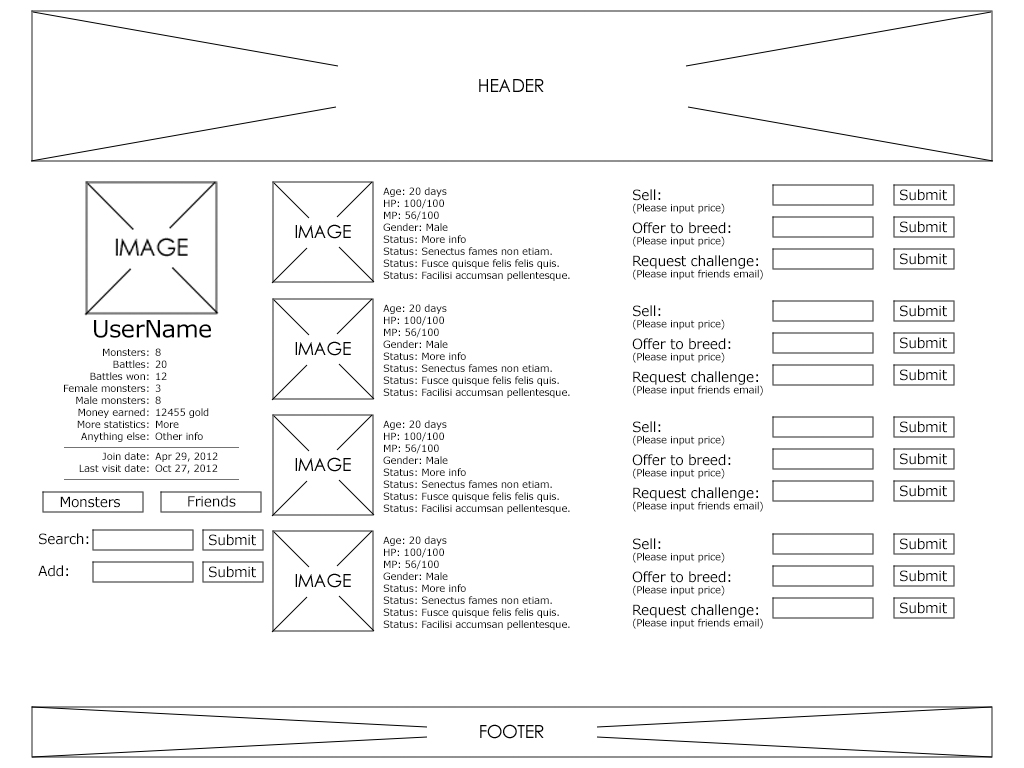
\includegraphics[width=\textwidth]{img/UI4.jpg}
\captionof{figure}{Version 1}

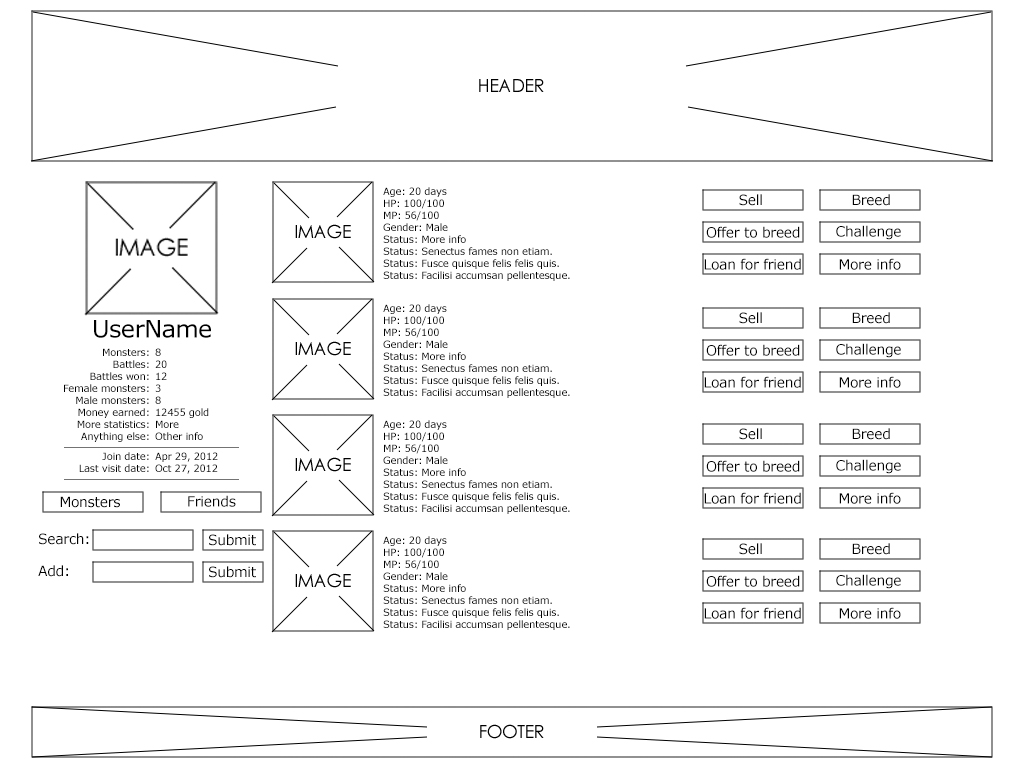
\includegraphics[width=\textwidth]{img/UI5.jpg}
\captionof{figure}{Version 2}

Each of the options to interact with the user's monster will bring up a pop-up menu where they can specify options. For example, if the user presses the 'Sell' button, the following pop-up will be displayed:

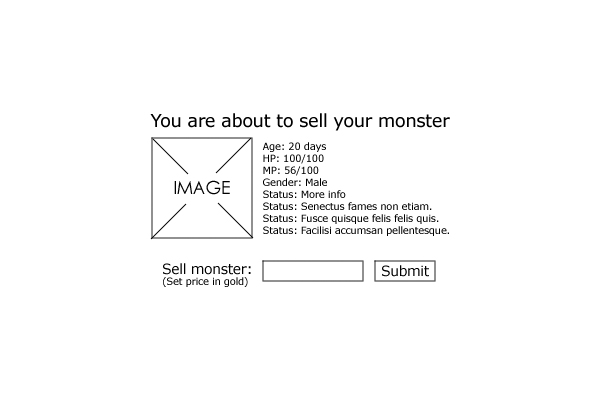
\includegraphics[width=\textwidth]{img/UI6.jpg}

Similarly, the Offer to breed button:

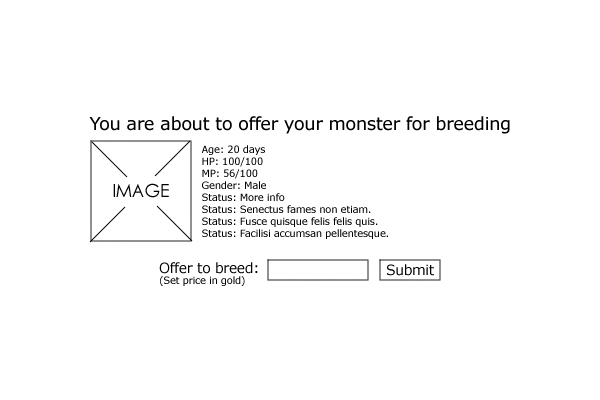
\includegraphics[width=\textwidth]{img/UI7.jpg}

Loan to friend button:

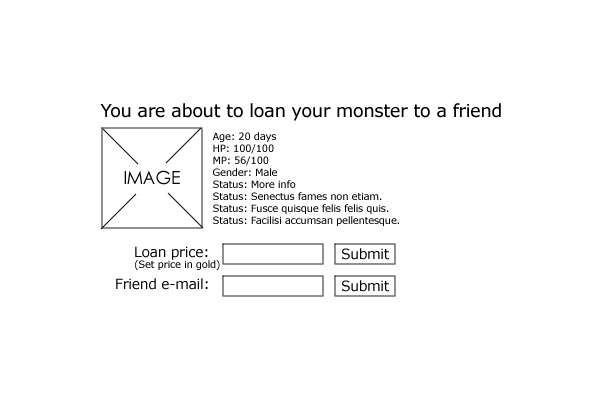
\includegraphics[width=\textwidth]{img/UILoan.jpg}
\clearpage

If the user clicks the 'Breed' option, they will have to choose another monster to breed with - this will be inputted into the form before clicking 'Submit':

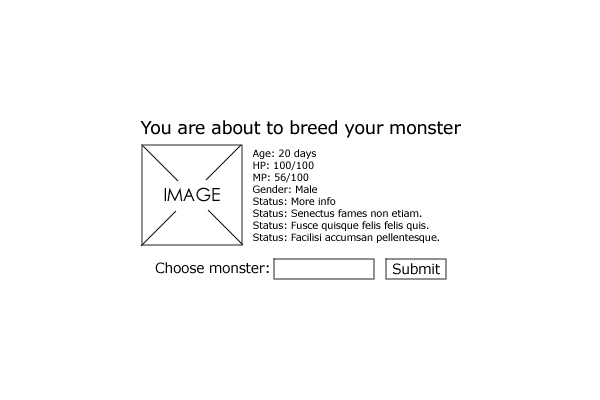
\includegraphics[width=\textwidth]{img/UI10.jpg}

If the user wants to challenge another monster, they have to input that friend's email address:

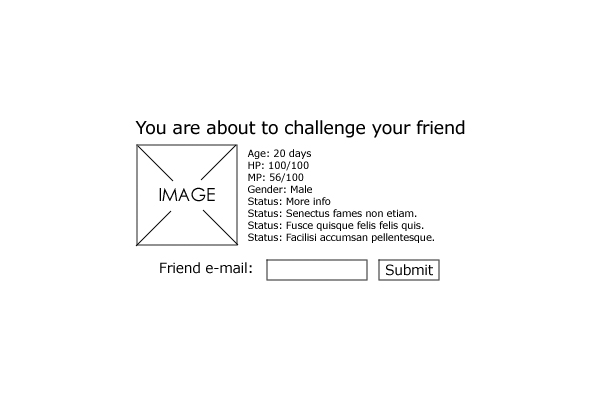
\includegraphics[width=\textwidth]{img/UI11.jpg}
\clearpage

There is also an option for finding out more information about each monster - here the user will be able to edit information:

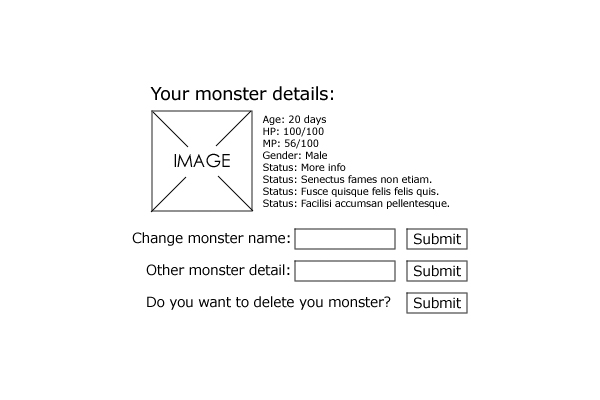
\includegraphics[width=\textwidth]{img/UI12.jpg}
\clearpage

Friends list:\\

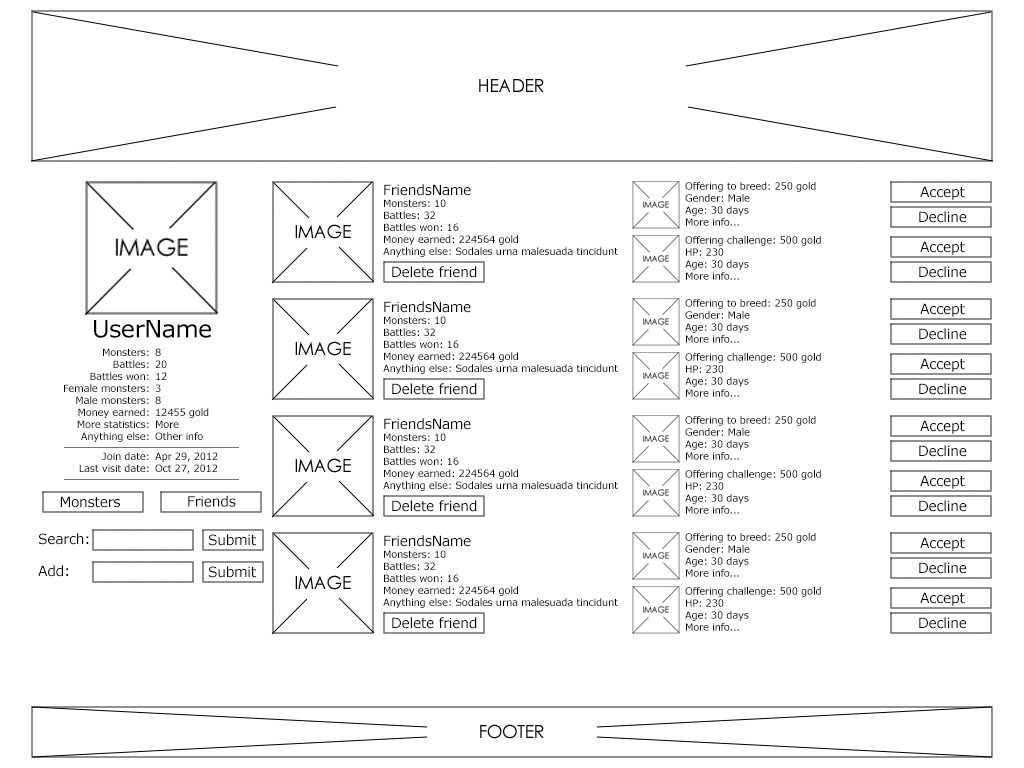
\includegraphics[width=\textwidth]{img/UI13.jpg}
\clearpage

The header should have links to personal settings profile as well as log out function:\\

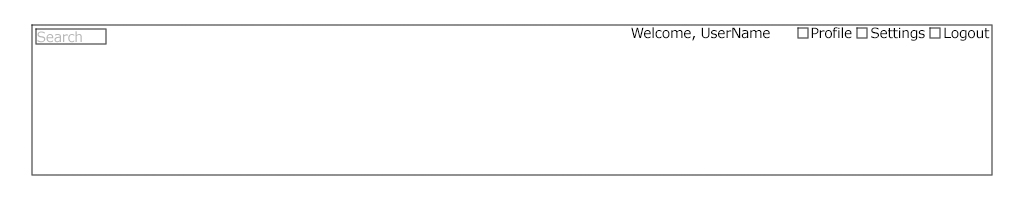
\includegraphics[width=\textwidth]{img/UIHeader.jpg}

Footer to contain copyright information and other links:\\

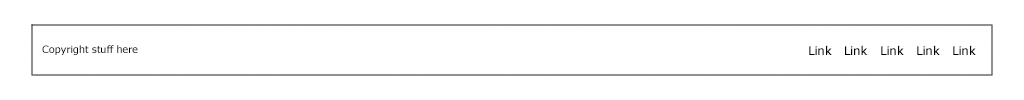
\includegraphics[width=\textwidth]{img/UIFooter.jpg}
\clearpage

The settings page allows the user to change their password, avatar and other personal information available for friends to see. Extra options for deleting the account, deleting and adding friends, etc.\\

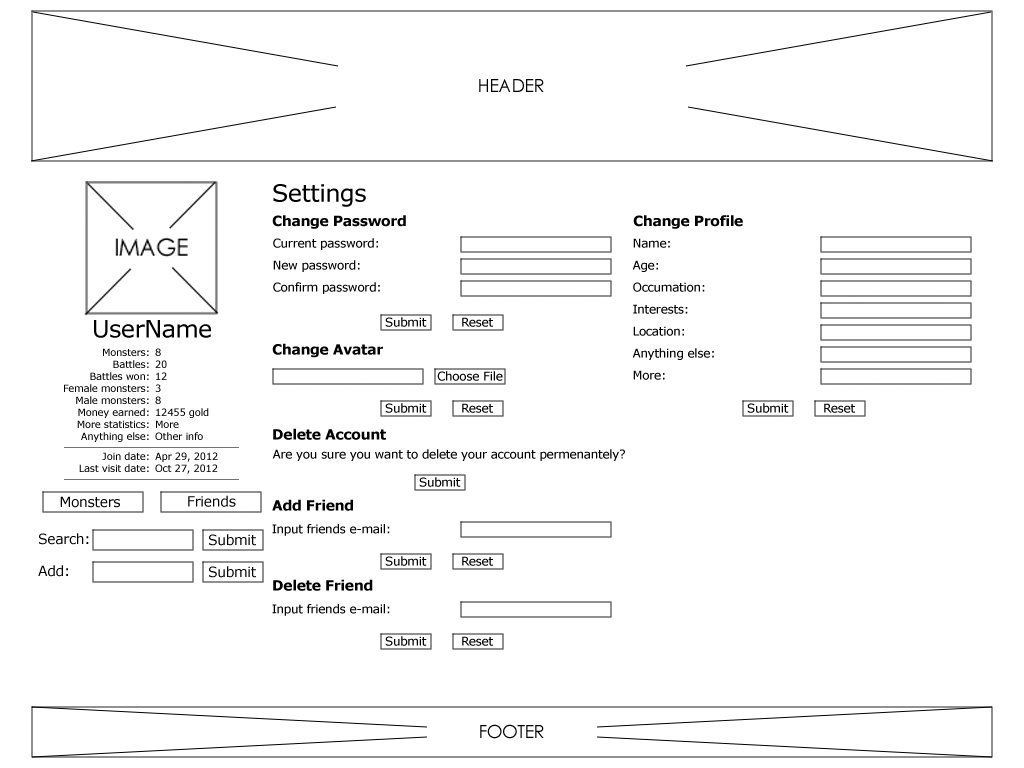
\includegraphics[width=\textwidth]{img/Settings.jpg}
\clearpage

%Scott - Gantt Chart
\section{Gantt Chart}

See Gantt chart on following page.
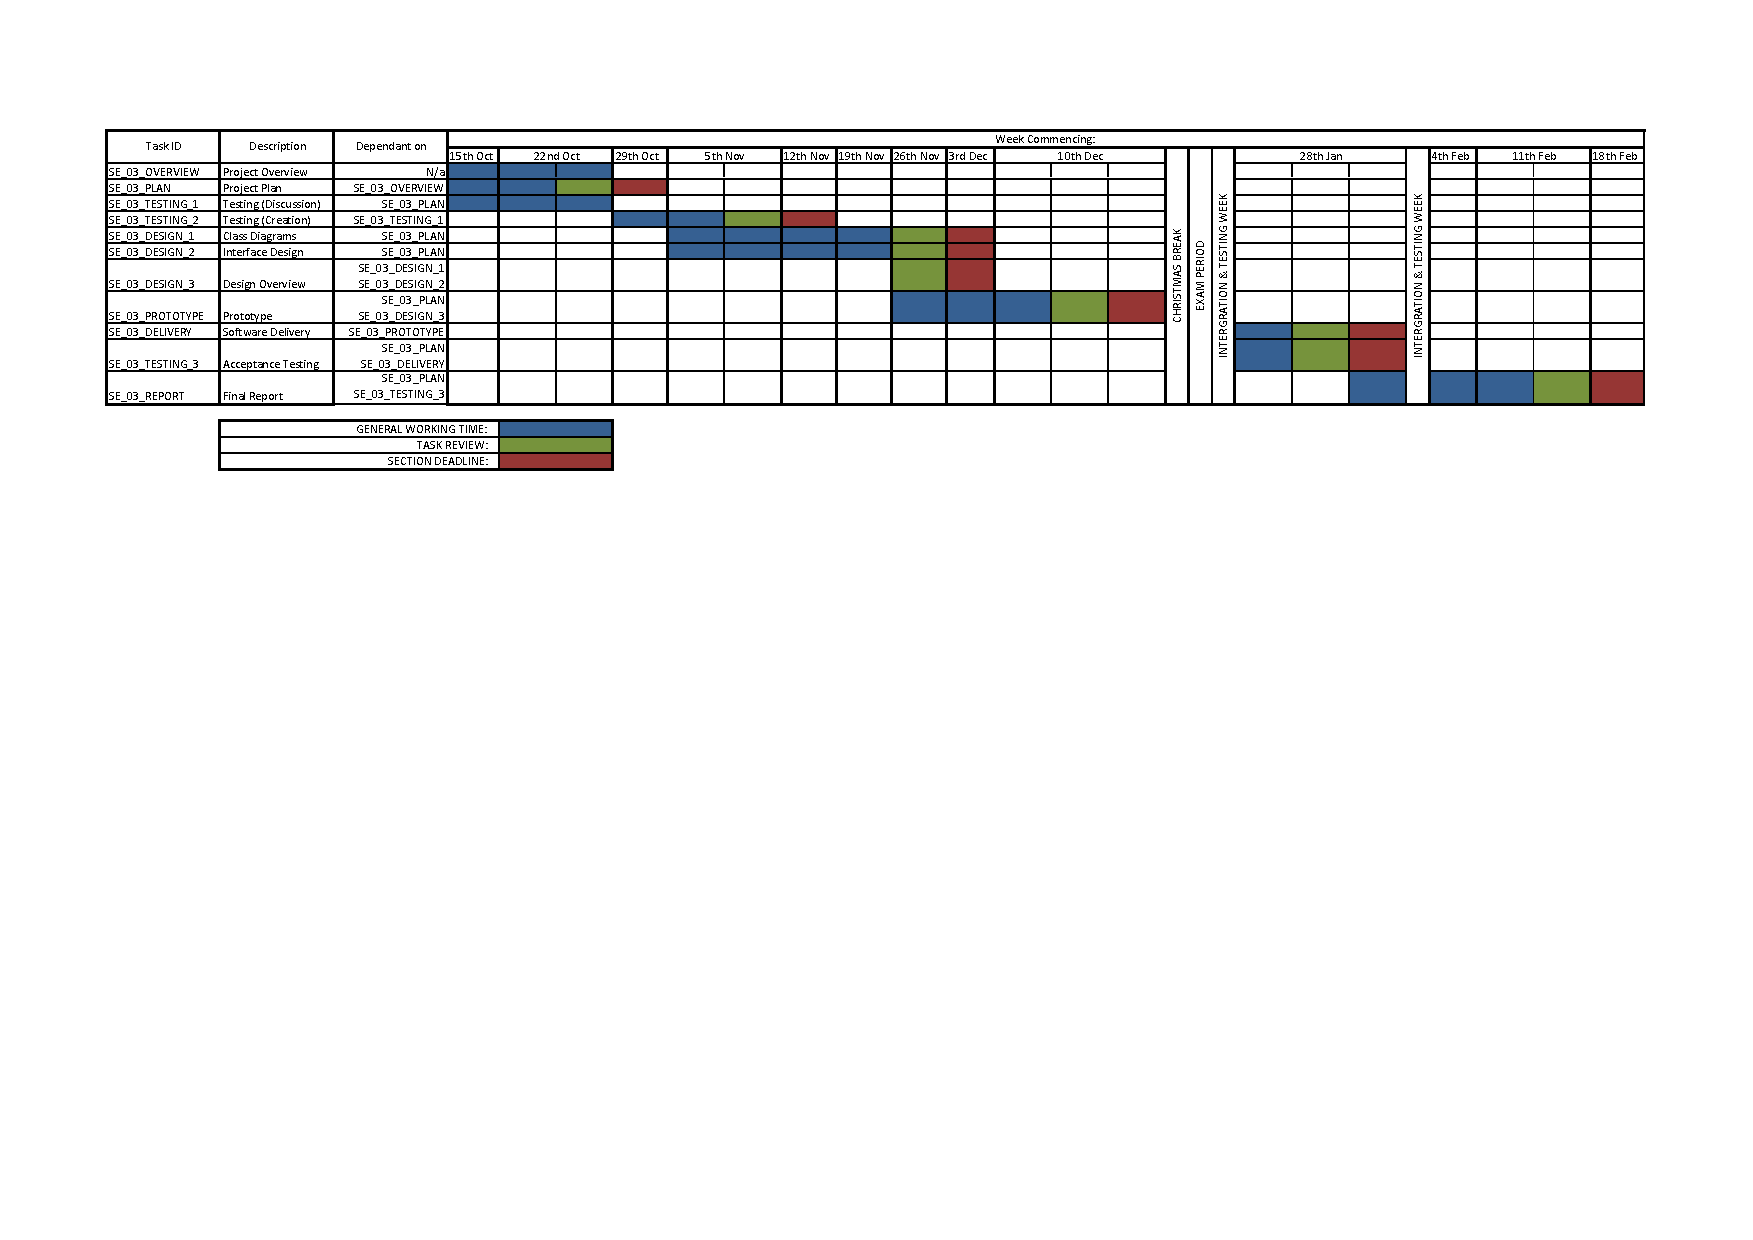
\includepdf[landscape=true]{img/Gantt2.pdf}
\clearpage

%Simon - Risk Analysis

\section{Risk Analysis}

\subsection{Scheduling issues}

Through the Gantt chart, all group members can see when each specific task is intended to be completed. However, estimates made in advance for each task to be completed can often be incorrect, or most commonly, group members may run into problems and need additional time to complete tasks. In the event of tasks running over their estimated time periods, a larger amount of tasks will need to be run in parallel so as to avoid running out of time for end of project tasks - such as testing and integration.

\subsection{Illness}

It is likely that, during the course of the project, group members may not be able to contribute towards the project due to illness. Unfortunately, it is impossible to know when group members will be absent, however it is important that measures are put into place to ensure that the project can still go forward and be completed. One method of doing so is the use of deputies - both the QA Manager and the Project Leader have deputies to avoid the project to carry on through absence of either member.\\

However, for other group members, deputies have not been chosen. Instead, the best way to combat the problem in these cases is to use the SVN regularly. If all project work is continuously backed up, different group members will be able to take over work originally started by another group member. This furthermore stresses the necessity to produce code that is well documented and commented - this should be practised anyway.

\subsection{Technical difficulties}

Although the group has agreed on specific release versions of software to use for compatibility reasons, technical problems within the code itself may still arise. If communication between programmers is poor, the expected result of one group member's algorithm (for example) may be different to the actual outcome, causing technical problems for the other group member working on that specific part of the project. To avoid this, it is suggested that group members produce code that is well commented and documented, and hold regular meetings with others concerned.

\subsection{Task allocation}

Although each group member has been given a broad role within the project, specific task allocation can become a problem when the wrong person is assigned the wrong task. For example, it would be pointless to ask the lead programmer to spend the majority of their time just testing other peoples' code. Furthermore, it is equally important to balance the amount of group members on each task, even when there are problems. Although some tasks may require more attention than others, the more people working on it at once will reduce the amount of time available to be spent on other equally important tasks.
\clearpage
\section{References}
[1] \textit{Software Engineering Group Project.} QA Plan.
Bernard Tiddeman. SE.QA.01. 1.8 Final. \\ \relax \\ \relax
[2] \textit{Software Engineering Group Project.} Project Plan Specification Standard.
Bernard Tiddeman. SE.QA.05B. 1.1 Final.
\clearpage
\section{Document History}
\begin{tabular}{|l | l | l | l | l |}
\hline
Version & CCF No. & Date & Changes made to Document & Changed by \\
\hline
1.0 & N/A & 26/10/2012 & First version created & SIE5\\
\hline
1.1 & N/A & 27/10/2012 & Title page edited and Risk Analysis added & SIE5\\
\hline
1.2 & N/A & 28/10/2012 & Gantt chart and User Interface section added & SIE5 \\
\hline
1.3 & 1 & 29/10/2012 & Corrected spelling, added revised Gantt chart & SIE5 \\
\hline
\end{tabular}

\end{document}